%\documentclass{beamer}
%\documentclass[c]{beamer}
\documentclass[t]{beamer}
%\documentclass[b]{beamer}
\listfiles

\mode<presentation>
{
% \usetheme[english]{KIT}
% \usetheme[usefoot]{KIT}
  \usetheme[deutsch]{KIT}

%%  \usefonttheme{structurebold}

  \setbeamercovered{transparent}

  %\setbeamertemplate{enumerate items}[circle]
  \setbeamertemplate{enumerate items}[ball]
}

\usepackage{babel}
\date{25.06.2019}
%\DateText

%\KITfoot{\parbox[t]{90mm}{\today:\qquad Dies ist eine sehr lange selbstdefinierte Fu\ss{}zeile -- Dies ist eine sehr lange selbstdefinierte Fu\ss{}zeile -- Dies ist eine sehr lange selbstdefinierte Fu\ss{}zeile}}

\usepackage{xcolor}
\usepackage[utf8]{inputenc}
\usepackage[TS1,T1]{fontenc}
\usepackage{array}
\usepackage{lipsum}
\usepackage{hyperref} 
\usepackage{listings}

\input{Code/my_c_style.tex}

\usepackage{glslListings}

\usenavigationsymbols
%\usenavigationsymbols[sfHhdb]
%\usenavigationsymbols[sfhHb]

\title[Aufbau einer modernen Rendering-Pipeline]{Aufbau einer modernen Rendering-Pipeline}
\subtitle{Von der Anwendung zum Bildschirm}

\author{Jonas Heinle}

\institute{Fakultät für Informatik - Lehrstuhl für Computergrafik - Institut für Visualisierung und Datenanalyse}

\TitleImage[height=\titleimageht]{Bilder/StormTrooper2Small.png}

\begin{document}

\begin{frame}
  \maketitle
\end{frame}

\begin{frame}
  \frametitle{Motivation}
  
  \begin{figure}[ht]
    \begin{minipage}[b]{0.45\linewidth}
        \centering
        \includegraphics[width=\textwidth]{Bilder/Kette.jpg}
    \end{minipage}
    \hspace{0.5cm}
    \begin{minipage}[b]{0.45\linewidth}
        \centering
        \includegraphics[width=\textwidth]{Bilder/Pipeline.jpeg}
    \end{minipage}
  \end{figure}
  
\end{frame}

\section{Motivation}
\begin{frame}
  \frametitle{Motivation}

  \begin{centering}
    \hspace*{0.5cm}\includegraphics[width=0.9\textwidth]{Bilder/cyberpunk_2077.png}
  \end{centering}
  
\end{frame}

\begin{frame}
  \frametitle{Motivation}

  \begin{centering}
    \hspace*{4.5cm}\includegraphics[width=0.25\textwidth]{Bilder/RenderingPipelineVereinfacht.png}
  \end{centering}
  \ref{Vulkan Pipeline}

\end{frame}

\section{Anwendung}
\begin{frame}
  \frametitle{Blenders Suzanne}
  \centering
  \includegraphics[width=\textwidth]{Bilder/Suzanne.png}
\end{frame}

\begin{frame}
  \frametitle{Anwendung}

  \vspace{1cm}
  \begin{figure}[ht]
    \begin{minipage}[b]{0.45\linewidth}
        \centering
        \includegraphics[width=\textwidth]{Bilder/ObjectData.png}
        \caption{Beispielhafte Objektdefinition}
    \end{minipage}
    \hspace{0.5cm}
    \begin{minipage}[b]{0.45\linewidth}
        \centering
        \includegraphics[width=\textwidth]{Bilder/MaterialDefs.PNG}
        \caption{Beispielhafte Materialdefinition}
    \end{minipage}
    
\end{figure}

\end{frame}

\begin{frame}
  \frametitle{Anwendung}
  \hspace*{3cm}\includegraphics[width=0.5\textwidth]{Bilder/kd_Baum.jpg}
  \ref{pic:kdtree}
  \begin{itemize}
    \item Beschleunigungsstrukturen BVH
    \pause
    \item Kollisionserkennung
    \pause
    \item Benutzereingaben
    \pause
    \item Kommuniziert mit Shadern (uniforms)
  \end{itemize}
\end{frame}

\section{Geometry Stage}
\begin{frame}
  \frametitle{Primitive Assembly}
  Zusammensetzung von Eckpunkten zu Primitiven (Linien,Drei-/Vierecke)
  \vspace{1cm}
  \begin{centering}
    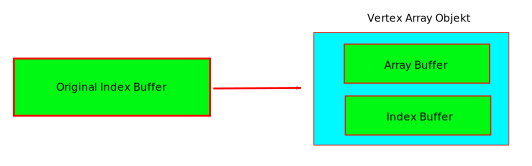
\includegraphics[width=\textwidth]{Bilder/PrimitiveAssembly.pdf}
  \end{centering}

\end{frame}

\begin{frame}
  \frametitle{Vertex Shader}
  \begin{centering}
    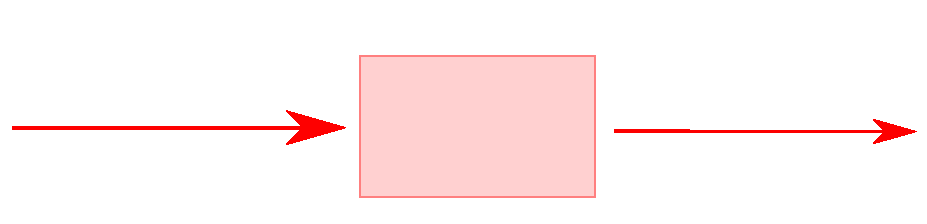
\includegraphics[width=\textwidth]{Bilder/VertexShader.pdf}
  \end{centering}
  \begin{itemize}
    \item jeder Eckpunkt wird für sich betrachtet
    \item andere Berechnungen möglich \ref{vertexshader_prozeduraleBewegung}
  \end{itemize}

\end{frame}

\begin{frame}
  \frametitle{Vertex Shader}
  \lstinputlisting[label = Shading im Geometry Shader, language=GLSL, caption={Beispielhafter Vertex Shader}]{Code/vertex_shader.c}
\end{frame}

\begin{frame}
  \frametitle{Tessellation}

  \vspace{2cm}
  \begin{centering}
    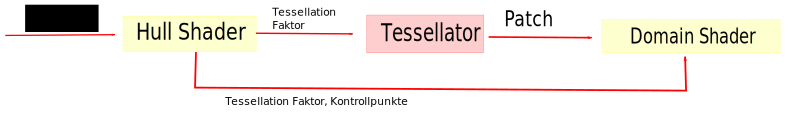
\includegraphics[width=\textwidth]{Bilder/Tessellation.pdf}
  \end{centering}

\end{frame}

\begin{frame}
  \frametitle{Tessellation}
  \vspace{1cm}
  \begin{centering}
    \includegraphics[width=\textwidth]{Bilder/Tessellation_Teapot.png}
    \ref{pic:Teapot}
  \end{centering}

\end{frame}

\begin{frame}
  \frametitle{Geometry Shader}

  \begin{center}
    Primitive (Punkt, Linie, Dreieck) werden vervielfacht, entfernt oder umgewandelt
  \end{center}
  \vspace{1cm}
  \begin{centering}
    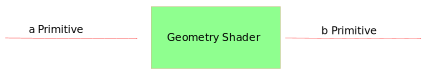
\includegraphics[width=\textwidth]{Bilder/GeometryShader.pdf}
  \end{centering}

\end{frame}

\begin{frame}
  \frametitle{Geometry Shader - Instanziierung}
  \begin{centering}
    \includegraphics[width=\textwidth]{Bilder/instancing-balloons.jpg}
  \end{centering}
  \ref{Geometry Instancing}
\end{frame}

\begin{frame}
  \frametitle{Geometry Shader und Shading}
  \lstinputlisting[label = Shading im Geometry Shader, language=GLSL, caption={Beispielhafter Geometry Shader}]{Code/geometry_shading.c}
\end{frame}

\begin{frame}
  \frametitle{Geometry Shader und Shading}
  \lstinputlisting[label = Shading im Geometry Shader, language=GLSL, caption={Beispielhafter Geometry Shader}]{Code/geometry_shading2.c}
\end{frame}

\begin{frame}
  \frametitle{Projektionstransformation}
  \begin{itemize}
    \item Vorbereitung der Projektion
    \pause
    \item Alle Punkte liegen innerhalb eines Einheitswürfels
  \end{itemize}
  \begin{center}
    \includegraphics[width=\textwidth]{Bilder/view_frustrum.png}
  \end{center}
  \ref{pic:view_frustum}
\end{frame}

\begin{frame}
  \frametitle{Clipping}
  \begin{itemize}
    \item Objekte bzw. Objektausschnitte, welche außerhalb des Sichtfensters liegen, verwerfen
    \item Algorithmus von Sutherland-Hodgman
    \item Reihenfolge sehr wichtig: Projektionstransformation, Clipping, View-Port-Transform
  \end{itemize}
  \begin{center}
    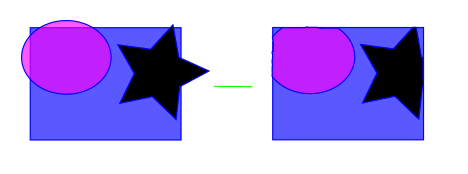
\includegraphics[width=\textwidth]{Bilder/clipping.pdf}
  \end{center}
\end{frame}

\section{Rasterisierung}
\begin{frame}
  \frametitle{Rasterisierung}
  \vspace{2cm}
  \begin{centering}
    
\includegraphics[width=\textwidth]{Bilder/Rasterisierung.pdf}
  \end{centering}
  \begin{itemize}
    \item Aufgabe: Finde heraus welche Geometrie bedeckt welchen Pixel zu welchen Anteil?
    \item (evlt.) Shading
  \end{itemize}
\end{frame}

\begin{frame}
  \frametitle{Rasterisierung}
  \begin{centering}
    \includegraphics[width=0.9\textwidth]{Bilder/RasterisierungSchaubild.png}
  \end{centering}
  \ref{pic:RasterisierungSchaubild}
\end{frame}

\begin{frame}
  \frametitle{Rasterisierung}
  \heading{Triangle Setup}
  \begin{itemize}
    \item nicht beeinflussbar vom Programmierer
    \pause
    \item Vorberechnungen; Interpolation Von Vertexattributen(Tiefe, )
    \pause
  \end{itemize}
  \heading{Triangle Traversal}
  \begin{itemize}
    \item alle Dreiecke werden durchgegangen
    \pause
    \item Fragmente werden erzeugt indem Pixel bestimmt werden die innerhalb des Dreiecks liegen
  \end{itemize}
  
\end{frame}

\begin{frame}
  \frametitle{Rasterisierung - Fragment Shader}
  \lstinputlisting[label = Shading im Geometry Shader, language=GLSL, caption={Beispielhafter Fragment/Pixel Shader}]{Code/fragment_shading.c}

\end{frame}

\begin{frame}
  \frametitle{Merging}
  \begin{itemize}
    \item Abschließendes Speichern der Farbgebung eines jeden Pixels im \textit{color buffer}
    \item Prüfung auf Sichtbarkeit mit Z-Buffer(Vorsicht bei Semi-Transparenz)
  \end{itemize}
\end{frame}

\section{Koordinatensysteme}
\begin{frame}
  \frametitle{Koordinatensysteme}
  \vspace{2cm}
  \begin{centering}
    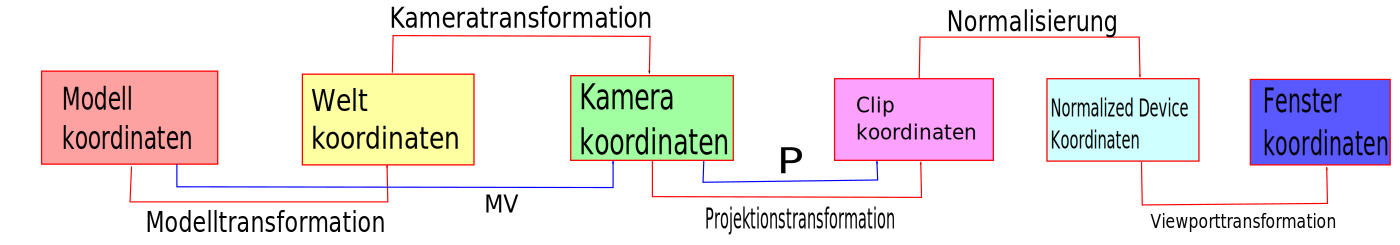
\includegraphics[width=\textwidth]{Bilder/Koordinatensysteme.pdf}
  \end{centering}

\end{frame}

\section{Compute Shader}
\begin{frame}
  \frametitle{Compute Shader}
  \begin{itemize}
    \item physikalische Simulationen, KI, spezielle Renderingverfahren
    \item SPMD
  \end{itemize}
  \begin{centering}
    \hspace*{2cm}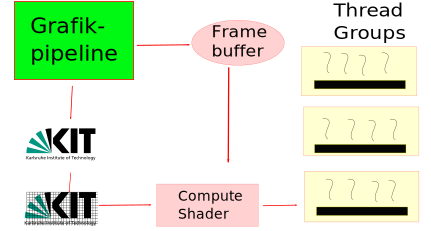
\includegraphics[width=0.7\textwidth]{Bilder/ComputeShader.pdf}
  \end{centering}

\end{frame}

\begin{frame}
  \frametitle{Compute Shader}
  \lstinputlisting[label = Shading im Geometry Shader, language=GLSL, caption={Beispielhafter Compute Shader}]{Code/compute_shader.c}
\end{frame}

\begin{frame}
  \frametitle{Compute Shader}
  \begin{centering}
    \hspace*{2cm}\includegraphics[width=0.7\textwidth]{Bilder/ComputeBlur.png}
  \end{centering}

\end{frame}

\begin{frame}
  \frametitle{Compute Shader}
  \begin{centering}
    \hspace*{2cm}\includegraphics[width=0.7\textwidth]{Bilder/ParticleSystem.jpg}
    \ref{Partikel System}
  \end{centering}
\end{frame}

\begin{frame}
  \frametitle{Compute Shader}
  \begin{centering}
    \hspace*{2cm}\includegraphics[width=0.7\textwidth]{Bilder/Haare.jpg}
  \end{centering}
\end{frame}

\section{Ausblick}

\begin{frame}
  \frametitle{Raytracing Unterstützung}

  \begin{centering}
    \hspace*{0.5cm}\includegraphics[width=0.9\textwidth]{Bilder/RayTracingPrinzip.png}
  \end{centering}
  \ref{Ray Tracing Prinzip}

\end{frame}

\begin{frame}
  \frametitle{Raytracing Unterstützung}

  \begin{centering}
    \hspace*{0.5cm}\includegraphics[width=0.9\textwidth]{Bilder/PICAPICA.jpg}
  \end{centering}
  \ref{pic:picapica}

\end{frame}

\begin{frame}
  \frametitle{Hybrides Rendering in \textit{PICA PICA}}

  \begin{centering}
    \begin{itemize}
      \item Transparenz und Durchsichtigkeit \textcolor{green}{Ray-Tracing}
      \pause
      \item Global Illumination \textcolor{green}{Ray-Tracing} \textcolor{blue}{Compute}
      \pause
      \item G-Buffer Layout \textcolor{red}{Rasterisierung}
      \pause
      \item Direkte Schatten \textcolor{green}{Ray-Tracing} \textcolor{red}{Rasterisierung}
      \pause
      \item Reflexionen \textcolor{green}{Ray-Tracing} \textcolor{blue}{Compute}
      \pause
      \item Direkte Beleuchtung \textcolor{blue}{Compute}
      \pause
      \item Post-Processing \textcolor{blue}{Compute}
    \end{itemize}
  \end{centering}
  \ref{pic:picapica}

\end{frame}

\begin{frame}
  \frametitle{Task/-Mesh Shaders}

  \begin{centering}
    \hspace*{0.5cm}\includegraphics[width=0.9\textwidth]{Bilder/NvidiaAsteroid.jpg}
  \end{centering}
  \ref{pic:asteroids}
\end{frame}

\begin{frame}
  \frametitle{Task/-Mesh Shaders}

  \begin{centering}
    \hspace*{0.5cm}\includegraphics[width=0.9\textwidth]{Bilder/meshlets_pipeline.png}
  \end{centering}
\end{frame}

\begin{frame}
  \frametitle{Fragen?}
  
  \begin{centering}
    \hspace*{0.5cm}\includegraphics[width=0.9\textwidth]{Bilder/Ende.jpg}
  \end{centering}
  \ref{pic:witcher}
  
\end{frame}

\section{Zum Nachschlagen}
\begin{frame}
  \frametitle{Interesse geweckt ...?}
  \heading{Weiterführende Literatur}
  
  \begin{enumerate}
    \item \href{http://www.brechpunkt.de/q2vkpt/}{Quake2 Real-Time Raytracing Project Q2VKPT}
    \item \href{https://developer.nvidia.com/rtx/raytracing}{NVIDIA RTX Ray Tracing}
    \item \href{https://www.nvidia.com/en-us/geforce/news/graphics-reinvented-new-technologies-in-rtx-graphics-cards/}{RTX}
    \item \href{https://www.pbrt.org/}{Physically Based Rendering}
    \item \href{https://www.heise.de/newsticker/meldung/Nvidias-Asteroids-Demo-zeigt-Mesh-und-Task-Shader-in-Aktion-4258243.html}{Heise about NVIDIA Asteroid Demo}
    \item \href{http://www.realtimerendering.com/}{Link to very much information!}
    \item \href{http://vulkan-spec-chunked.ahcox.com/ch09.html}{Vulkan Rendering Pipeline}\label{Vulkan Pipeline}
    \item \href{https://developer.nvidia.com/discover/ray-tracing}{Ray Tracing}
    \item \href{https://dl.acm.org/citation.cfm?id=515351}{Vertex Shader Prozedurale Bewegung}\label{vertexshader_prozeduraleBewegung}
  \end{enumerate}
\end{frame}

\begin{frame}
  \frametitle{Links}
    \heading{Bilder}
    \begin{itemize}
      \item \href{https://arstechnica.com/gaming/2018/03/star-wars-demo-shows-off-just-how-great-real-time-raytracing-can-look/}{Titelbild}
      \item \href{https://variety.com/2019/gaming/news/cd-projekt-red-cyberpunk-2077-transgender-image-1203242424/}{Cyberpunk 2077}
      \item \href{https://www.karabiner-und-mehr.de/kamero-wallet-chain-schwere-kette-51cm-edelstahl-rostfrei-walletchain-kette-fuer-die-geldboerse-hosenkette.html}{Kette}
      \item \href{https://medium.com/@timhberry/terraform-pipelines-in-jenkins-47267129ff06}{Pipeline}
      \item \href{https://www.ea.com/seed/news/seed-project-picapica}{SEED's Project \textit{PICA PICA}} \label{pic:picapica}
      \item \href{https://devblogs.nvidia.com/using-turing-mesh-shaders-nvidia-asteroids-demo/}{NVIDIA Asteroid Scene} \label{pic:asteroids}
      \item \href{https://www.youtube.com/watch?v=NxKSMz6dcTA}{Witcher Endslide} \label{pic:witcher}
      \item \href{https://unity3d.college/2017/04/25/unity-gpu-instancing/}{Geometry Shader Instanziierung} \label{Geometry Instancing}
      \item \href{http://www.realtimerendering.com/Real-Time_Rendering_4th-Real-Time_Ray_Tracing.pdf}{Ray Tracing Prinzip} \label{Ray Tracing Prinzip}
      \item \href{https://www.geforce.co.uk/games-applications/pc-applications/fermi-hair-demo}{Haare mit Compute Shader}
      \item \href{https://chetanjags.wordpress.com/2014/04/15/gaussian-filter-using-compute-shader/}{Blur}
    \end{itemize}
    
    \vfill
    \mbox{}


\end{frame}

\begin{frame}
  \frametitle{Links}
    \heading{Bilder}
    \begin{itemize}
      \item \href{https://subscription.packtpub.com/book/game_development/9781789342253/7/ch07lvl1sec74/tessellating-a-3d-surface}{Teapot} \label{pic:Teapot}
      \item \href{https://www.keithlantz.net/2013/04/kd-tree-construction-using-the-surface-area-heuristic-stack-based-traversal-and-the-hyperplane-separation-theorem/}{kd-Baum}\label{pic:kdtree}
      \item \href{https://docplayer.org/41341773-Computer-graphik-i-polygon-scan-conversion-triangulation-filling-etc-g-zachmann-university-of-bremen-germany-cgvr-informatik-uni-bremen.html}{Rasterisierung Schaubild}\label{pic:RasterisierungSchaubild}
      \item \href{http://www.songho.ca/opengl/gl_projectionmatrix.html}{View Frustum} \label{pic:view_frustum}
    \end{itemize}
\end{frame}

\begin{frame}
  \frametitle{Links}
  
  \heading{Videos}
  
    \begin{enumerate}
      \item \href{https://www.youtube.com/watch?v=LXo0WdlELJk}{SEED's Project \textit{PICA PICA}}  
      \item \href{https://www.youtube.com/watch?v=CRfZYJ_sk5E}{Nvidias Asteroids Mesh Shaders Demo}
      \item \href{https://www.youtube.com/watch?v=40Mfvof4OS8}{Particle System} \label{Partikel System}
      \item \href{https://www.youtube.com/watch?v=AdabPy6xQ8A}{Instancing Unreal Engine}
    \end{enumerate}

\end{frame}

\end{document}
